\documentclass[12pt,letterpaper,oneside]{memoir}

%%% Resets
% memoir defines footruleskip, we want fancyhdr's
\let\footruleskip\undefined
\DisemulatePackage{setspace}

%%% Packages
\usepackage{caption}
\usepackage{enumitem}
\usepackage{fancyhdr}
\usepackage{graphicx}
\usepackage{hyperref}
\usepackage{pdfpages}
\usepackage{wrapfig}

%%% Headers/Footers
\pagestyle{fancyplain}
\fancyhf{}
\fancyheadoffset[r]{.01in}
\lhead{\textit{\thetitle}}
\rhead{\theauthor}
\rfoot{\thepage}
\fancypagestyle{plain}{
  \fancyhf{}
  \renewcommand{\headrulewidth}{0pt}
  \renewcommand{\footrulewidth}{0pt}
}

%%% Font
\renewcommand\rmdefault{ptm}
\renewcommand\ttdefault{pcr}

%%% Spacing
\usepackage[top=1.5in, bottom=1.5in, right=1.5in, left=1.5in]{geometry}

%%% Commands
\newcommand\secdiv{
  \begin{center}
    \S
  \end{center}
}

%%% Title
\title{New American Absinthe}
\author{Madison Jesse Scott-Clary}
\date{April 1, 2016}

\begin{document}
  \maketitle

  \noindent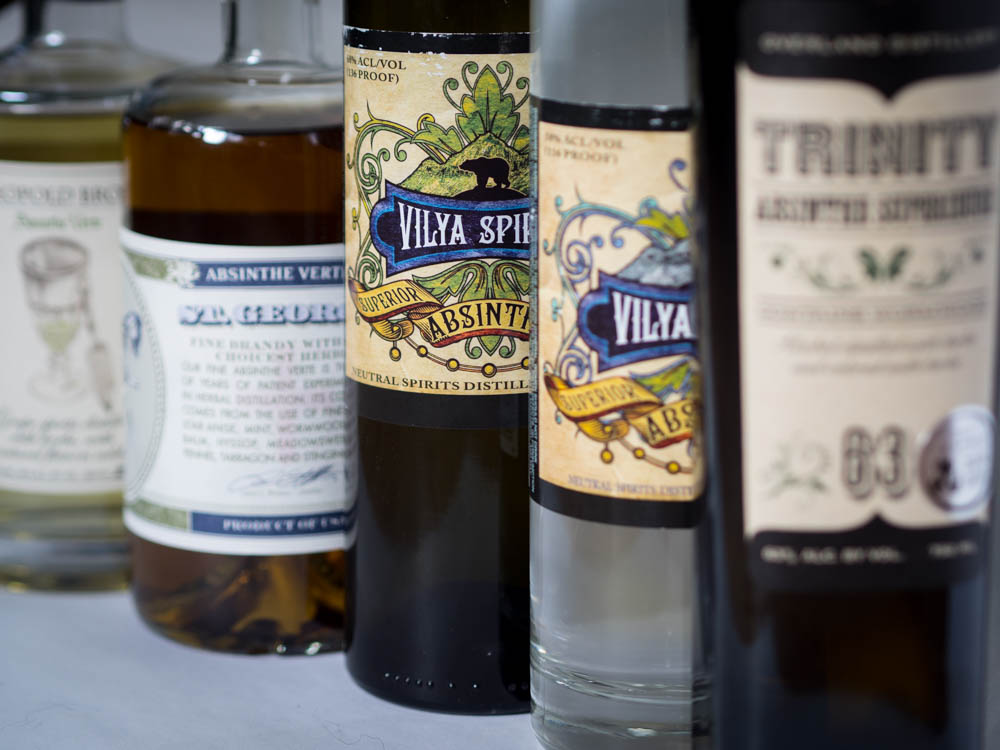
\includegraphics[width=\linewidth]{../../assets/tasting/naa-all.jpg}

  The weather is finally starting to turn.

  Well, I say finally like this winter hasn't been a rollercoaster, when it comes to weather.  We'd get a foot and a half of snow, then be back up in the 50s and 60s later in the week.  It makes it difficult to pick drinks, really.

  Over the winter, I tend toward darker, warmer drinks, such as heavy red wines, scotches, and heady mixed drinks without carbonation; if I'm going to have something carbonated, it's more likely to be a sweet ale than anything.  When it's hot outside during the summer, that's when I bust out the bubbles -- bubbly and Collinses and mojitos and gin-and-tonics -- and cold-as-hell mixed drinks (5The Aviation is a perennial favorite).  Autumn is reserved for brandy, lighter reds, and creamy mixed drinks.

  Spring?  Spring is for Absinthe.

  There's something about the tumult of flavors and scents involved in absinthe that fit the tumultuous weather so well.  When it's snowing out, you can feel the strength of the drink warming you from within, and when it's bright and sunny, you can revel in the refreshing rhythm of anise-fennel-wormwood-hyssop that goes with each sip.

  There's been a resurgence of good absinthe on the market over the last decade, and it's been fascinating to watch and taste.  It's hardly surprising, watching the trajectory of craft brewing and distilling over the last two decades.  At my old house, I was a bike ride from six breweries (Equinox, Coopersmith's, New Belgium, Fort Collins,  Odell's, Funkwerks) all in a row, leading to the pastime of brew tours that take up all Saturday.

  With the opening of Dancing Pines, Overland, and The Copper Muse local distilleries in the last few years, the distilling industry has clearly followed suit.

  And, always surrounded by so much mystique, it's easy to see why so many have picked up absinthe as an offering.

  \secdiv

  \section*{An Introduction to Absinthe}

  I spent a lot of time online when I was younger.  I still do, of course, but not nearly to the extent that I used to.  I spent my whole life online or waiting until the point when I could get back online.  I dated online, surrounded myself with online friends, and read and read and read.

  What I would read and get obsessed over would vary greatly.  For a while, I was into martial arts, then it was cooking, then it was constructed languages.  These would come into my life from those around me and wind their way around my every waking moment, occupying all of my thoughts.  None of them go away completely, though they might fade.

  During a few months in about 2005 and into 2006, that fascination was absinthe.  The roots of it come from several friends online who were desperately seeking new highs and better ways to get fucked up.  Absinthe, they had decided, would do nicely, because it would make you see shit.  It was all kind of muddy, they didn't really have their own reasoning nailed down.

  All they were worried about, really, was thujone.  They wanted something to really fuck them up, so they bought the strongest Czech absinthe (often spelled without the `e', absinth) that they could find.  These were usually uniquely shaped bottles filled a quarter of the way full with wormwood leaves, the primary source of thujone, and industrial grade alcohol.

  I shrugged a bought a relatively cheap bottle.  Absinth, King of Spirits, it declared itself.

  It was vile.

  Okay, it was worse than vile.  It was undrinkable, which is good because it was likely poisonous to boot.

  A few years prior, I had picked up the first in a trio of books by Dale Pendell, the \textit{Pharmako} trilogy.  The books themselves were investigations and musing on plants of power -- that is, plants that were able to exert power over human lives, whether that meant individually through an interesting biological reaction, or on a grander scale such that they shaped whole societies.

  I had leafed through the chapter on \textit{Artemisia absinthum} without too much interest countless times before, but now I reread it with greater interest.  \textit{Artemisia absinthum}, wormwood, plays only a small part in absinthe itself, the history of which is long and colorful.  The more I read, the less it seemed like what I had tried had been absinthe at all, but was simply dreck created to get a few bucks out of kids looking for a thrill.

  \begin{wrapfigure}{r}{0.5\linewidth}
    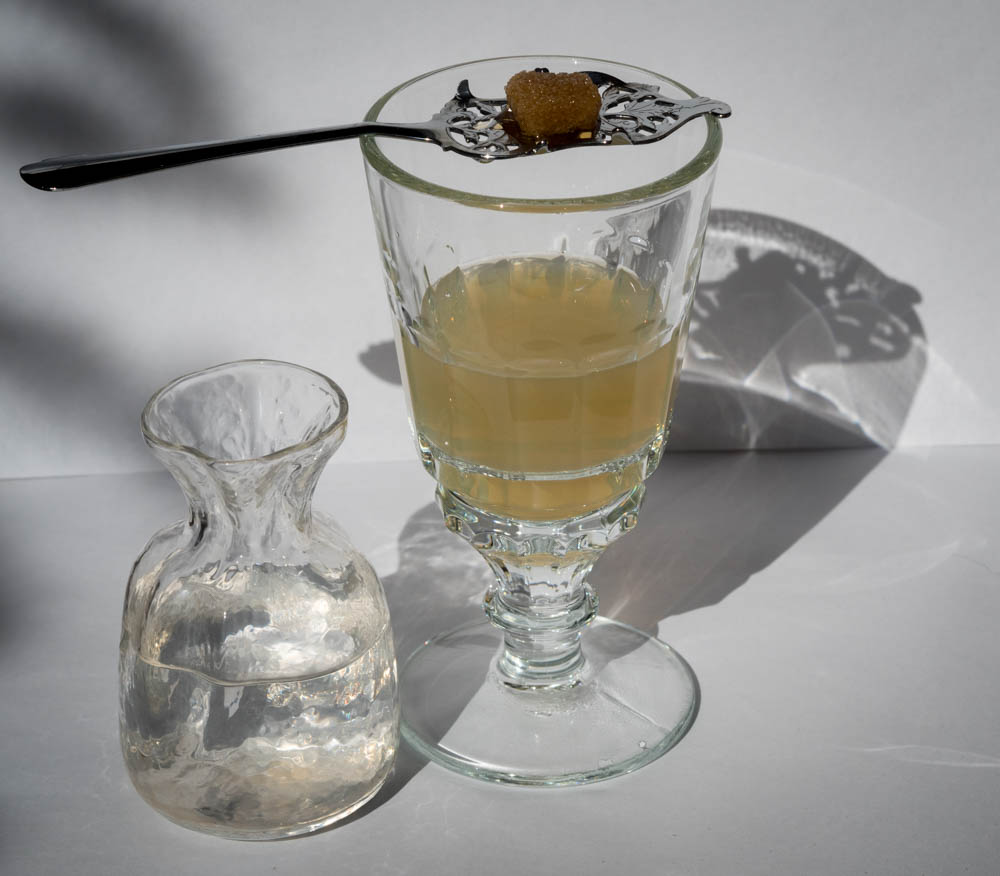
\includegraphics[width=\linewidth]{../../assets/tasting/naa-sugar.jpg}
    \textit{Sweetening absinthe with sugar.}
  \end{wrapfigure}

  Real absinthe is much more complex, and much more beautiful, than simply wormwood and ethanol.  There was in fact an entire world hidden beneath the surface of this topic.  This also helps to explain my interest in tea of late, as well.  Finding out that the more one looks into some topic, the more there is to find about it, is very appealing to me.  I love finding all of the ways in which things can be explored.

  So I moved on from my cheap Czech absinthes to researching absinthes more worthy of the name.

  I wound up finding my way to another site, one more focused on the types of absinthes that I had spent so much time reading about.  I came away with a few purchases -- a few less expensive 750ml bottles and a few sample bottles of some pricier, but more highly rated absinthes -- and waited impatiently for the shipment to arrive.  I was not without some trepidation, as I was only nineteen or twenty at the time, and if I had to sign for the bottles, I would be quite out of luck.  Alas, I was lucky, and DHL simply dropped the well-packed bottles on our stoop.

  The first two absinthes I tried were both from Distillerie Paul Devoille.  I got both the Verte de Fougerolles and Blanche de Fougerolles absinthes.

  Absinthe can be divided up into two general categories, of verte and blanche.  Both follow the same production steps, which I'll outline a little later on, but the verte style has an additional coloring step, where some select herbs are macerated in the clear product to add a bit of additional flavor and the green color that everyone associates with absinthe.

  Both of these were wonderful introductions to the world of absinthes, which I was quickly diving into.  They were complex, leading with anise, then delving into wonderful worlds of various different herbal flavors.  The verte was a little more peppery, I remember, than the blanche, and had a bit more of a fennel flavor to it.  I was hooked.

  After that, I got to try the samples from Jade, produced at the Combier Distillery in Saumur, France.  These went above and beyond even the Fougerolles absinthes in a big way.  Of note was the VS 1901 absinthe, which is one of the highest rated among new-production absinthes out there.  There was simply the perfect balance of sweet and herbal, anise and fennel and coriander.  To this day, it remains my absolute favorite absinthe, and I have a full bottle kept on the rack for a special occasion.  I won't wax too rhapsodic about it, however, as this is a story about new American absinthes.

  The first truly American absinthe that I had was produced by Leopold Bros., based out of my hometown of Denver, Colorado.

  \secdiv

  \section*{Leopold Bros. Absinthe Verte}

  Leopold Bros. absinthe is an interesting one.  \href{http://www.leopoldbros.com/}{The Leopold Bros. Distillery} first came to my attention through their blackberry flavored whiskey, an unoaked whiskey flavored with blackberry syrup.  It's a delightful combination that wound up in a drink at my local bar, Elliot's.  I ran to the store to pick some up after learning about the ingredients of the drink, and right there next to it on the shelf was the Leopold Bros. absinthe.

  I hadn't been drinking absinthe in quite a while -- I'd run out of my initial order of french absinthes, and didn't really want to pick up any more for the outrageous international shipping costs.  I grabbed a bottle of this on a whim and took it home.

  \begin{wrapfigure}{l}{0.4\linewidth}
    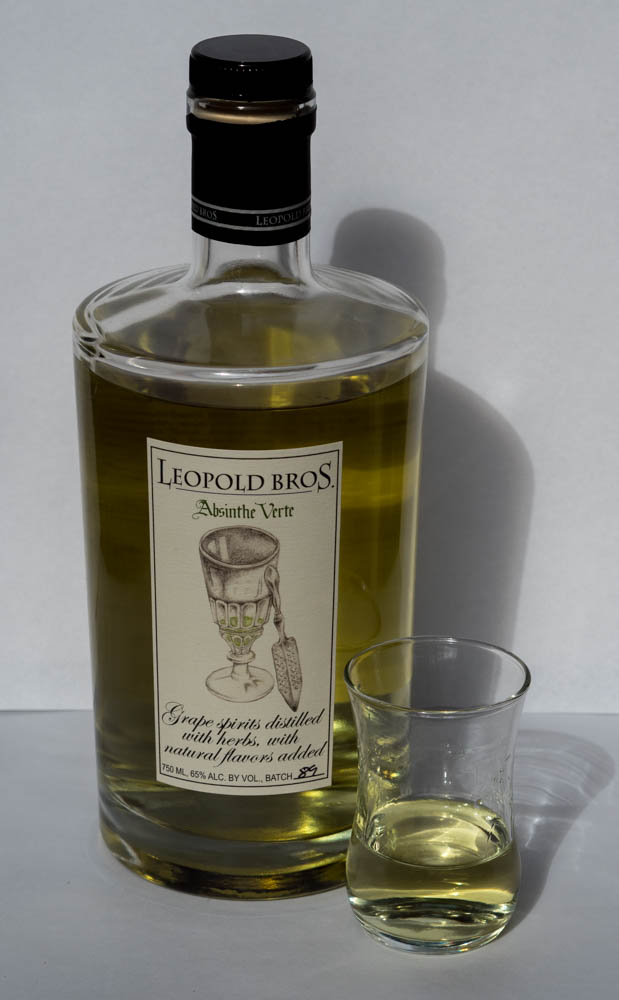
\includegraphics[width=\linewidth]{../../assets/tasting/naa-leopold.jpg}
  \end{wrapfigure}

  I was greeted by a very strange absinthe.  It turns out that Leopold Bros. had been more experimental with their first batches, and it wasn't until batch 15 that they settled on their current formula.  In fact, the batches differ so much, that they are rated as separate products in the Wormwood Society reviews: \href{http://www.wormwoodsociety.org/index.php/component/content/article/20-absinthe-brand-reviews/traditional-absinthe/577-leopold-brothers-absinthe-verte-batches-1-14}{batches 1-14} and \href{http://www.wormwoodsociety.org/index.php/component/content/article/20-absinthe-brand-reviews/traditional-absinthe/439-leopold-brothers-absinthe-verte-batches-15}{batches 15+}.

  I'm reviewing batch 89 here, but it's worth noting some of the characteristics of that first bottle, from batch 4.  The color was more of a drab color, closer to the color that shows up in the St. George absinthe mentioned later.  The taste was intriguing.  It lead with anise and fennel, but there was a definite note of oregano that I found rather enjoyable.  It was a good drink, though perhaps not a very accurate absinthe.

  On to this batch, though!

  The color of this batch is fairer, cleaner looking than the olive of the earlier batches.  As far as absinthes go, it is still on the lighter side and little yellow.  It's reminiscent of dried herbs, rather than fresh, though this is hardly a fault.  I'll explain more about where the color in verte absinthes comes from in a bit.

  Straight, the spirit smells primarily of fennel (a sort of green, licorice scent) and anise (a more pure anise scent), but that is soon overwhelmed with hot alcohol.  The grape spirit base of this drink is evident, in a calming warmth -- the cuts on the base spirit are fine, with no odd notes of solvents or fusel oils.  The emptied nosing glass, allowed to evaporate for a minute or so, starts to show more complexity, with fresh hyssop and perhaps angelica showing through.

  One doesn't drink absinthe straight, however.  This one clocks in at 68\% alcohol by volume (174 proof), which would make for quite the intense drink.  Instead, one dilutes the alcohol with water, one part absinthe to anywhere from three to five parts water.  In the process, the absinthe louches.

  Some of the herbs used in production of absinthe contain alcohol soluble compounds which have one hydrophobic (water-hating) end and one hydrophilic (water-loving) end which may be a separate surfactant.  When water is added, these compounds clump together with their hydrophobic ends facing in and their hydrophilic ends facing outward, leading to the cloudiness that one sees in the final drink.  The same can be seen with ouzo and raki.  These terpenes come primarily from anise and star anise, as well as from fennel and coriander, and form an emulsion with the water.

  The Leopold Bros. absinthe louches quick and thick at 3:1 water to absinthe, despite it's pale color.  And, despite the yellow tinge to the undiluted absinthe, the louche is creamy and green, like the center of an Andes mint.  It's a very fresh color, to counter the dried-herb appearance.

  Although it's not to my tastes, absinthe is often drunk with sugar.  This is done by placing a slotted absinthe spoon across the opening of the glass, placing a sugar cube on the spoon, and slowly dripping water over the sugar cube to dissolve it into the drink.  This is done because sugar is not readily soluble in alcohol of this strength.

  Without sugar, the absinthe is bracing, refreshing, and herbal.  At the fore is a sweet anise note that fades into delightful herbal flavors, leading with hyssop, then fading to a wonderful bitter wormwood.  The sweetness of the anise soon coats the mouth and fades into a fresher fennel taste.  After swallowing, the hyssop herbal flavors and the wormwood bitterness combine to leave your mouth feeling cool, and the body refreshed.

  When prepared with sugar, the absinthe differs in that the fresh, astringent hyssop flavor turns almost to mintiness, bringing that cooling feeling to the tongue and lips sooner than without sugar.  Additionally, the bitterness of the wormwood is covered up as the sugar blends with the anise and fennel to make for a more candy-like experience, rather like those sugar-coated fennel seeds one sees at Indian restaurants, though less earthy than that implies.

  \secdiv

  \section*{A Short History of Absinthe}

  \begin{wrapfigure}{l}{0.4\linewidth}
    \vspace{-20pt}
    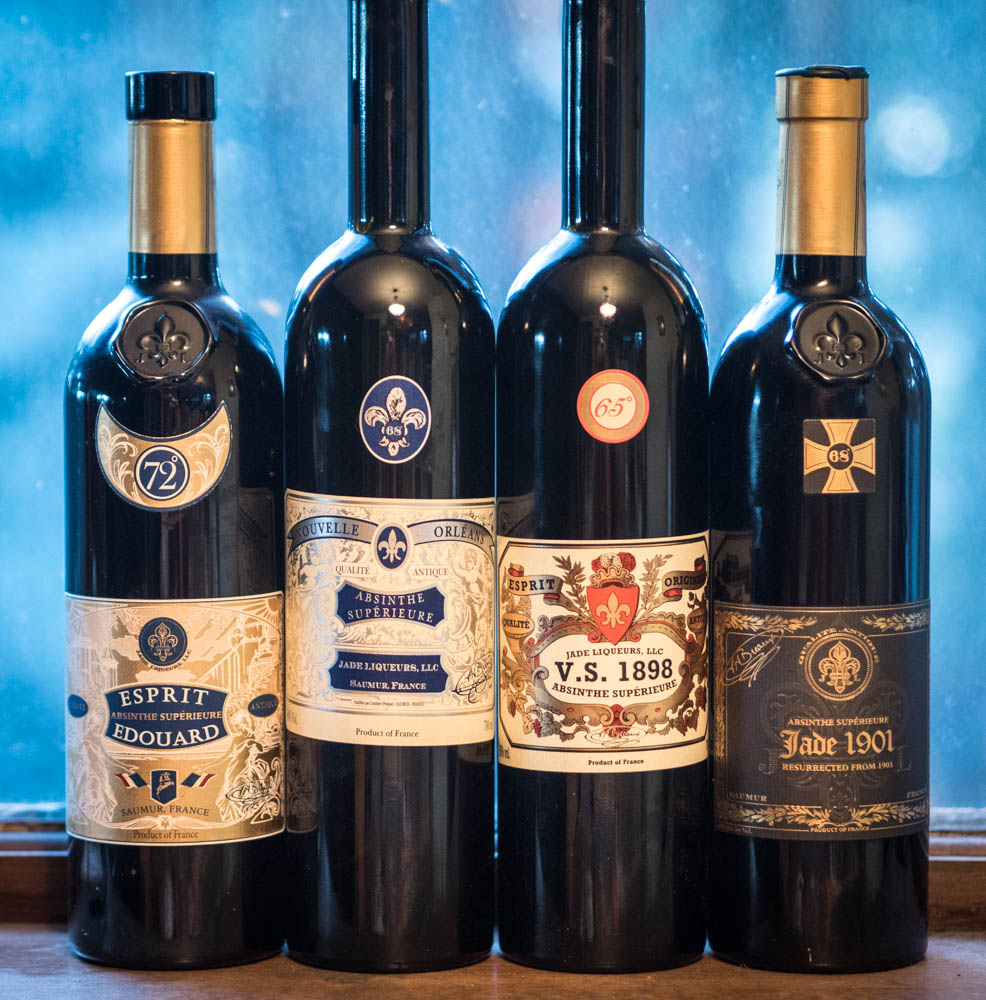
\includegraphics[width=\linewidth]{../../assets/tasting/naa-french-absinthes.jpg}\\
    \textit{From France, new takes on vintage absinthes from Jade Liquors.}
    \vspace{-50pt}
  \end{wrapfigure}

  As is perhaps obvious, absinthe has a storied history.  Although much of this can be attributed to folklore, absinthe was originally created in Switzerland by one Dr. Ordinaire, who first sold the concoction as a healthful tonic.  From Ordinaire, the recipe passed to his housekeeper, and from his housekeeper to her two daughters, who continued to sell the supposed cure-all.

  Although impressed by the curative powers of absinthe, one Major Dubied was more taken by it's aphrodisiacal qualities, and he purchased the recipe from the two women.  From there, Dubied passed the recipe on to his son-in-law as a wedding gift, and Henri-Louis Pernod began manufacturing absinthe on a larger scale in 1805.

  For a long time, absinthe remained a health tonic of sorts, used by French soldiers in Algeria to help prevent malaria (a claim not without merit), as well as for all of the benefits of wormwood itself.  Wormwood, along with many in the Artemisia genus, does wonders at repelling insects, as a vermifuge, and as a febrifuge, and had been taken with wine for thousands of years prior to the invention of absinthe for its medicinal properties.


  When the soldiers, who had been drinking absinthe for years, brought the liquor back to Paris, it took off, notably among those involved with art and literature:

  \begin{quotation}
    Manet painted absinthe themes, and his friend Charles Baudelaire drank absinthe[\ldots].  Verlaine and Rimbaud seem to have drunk absinthe more or less continuously.  Van Gogh drank it.  Poe drank it.  Degas drank absinthe in the cafes and then painted absinthe, stirring up a scandal in London.  There was something about light seen through an absinthe intoxication that seemed to feed the impressionists.  Henri Toulouse-Lautrec drank absinthe and painted it frequently.  Paul Gaugin liked absinthe and was somehow able to continue drinking it even in Tahiti.  Alfred Jarry called absinthe ``Holy Water'', and his friend Pablo Picasso painted pictures of absinthe a number of times.  Jack London liked absinthe.

    What other psychotropic concoction, excepting perhaps wine, has produced as large a body of laudatory poems in the last two thousand years as has absinthe?

    \vspace{14pt}
    \noindent--- Dale Pendell, in \textit{Pharmako/Poeia}
  \end{quotation}

  So when did the tide turn against absinthe?

  There were two events that worked against absinthe as time went on.  The first was the defense of a man named Lanfrey in 1906, used in his trial for the murder of his wife and family.  He drank a bottle of wine, a bottle of brandy, and several glasses of absinthe every day, but claimed that it was absinthe which made him crazy enough to kill his family.  Unlike the famed ``Twinkie defense'' used in the murders of Harvey Milk and George Moscone, the jury didn't buy it, and Lanfrey was convicted.  However, this served as fuel for the growing temperance movement.

  The second event was World War I.  As though confused as to why the troops were failing, charging head on against machine guns, absinthe was banned in France by the military.  The officers were confused as to why the troops didn't have enough ``vital spirit'', so absinthe took the blame.  Its downfall had been coming, however, as the French soldiers picked up a taste for cocktails and mixed drinks -- rather than absinthe -- from their American counterparts.

  Absinthe was later made legal again, and has, in fact, never been made wholly illegal in the USA, where I'm writing this article.  What \textit{was} up for debate, though, was the effects of thujone on the body.  Coming primarily from wormwood, lawmakers and regulators latched onto thujone as the so-called active ingredient in absinthe.

  The effects of thujone in large doses are primarily cognodysleptic, closer to that of marijuana than any supposed hallucinogenic activity (though, curiously, dogs injected with wormwood extract have been seen to bark at blank walls, as though indeed hallucinating -- yet how many of us are going to inject absinthe?).

  This is curious, however, given the dangers of thujone.  On average, wormwood contains about 1.5\% essential oils by weight, and only 0.15\% thujone by weight.  In a common older recipe of, say, thirty grams of wormwood per liter and 100\% extraction, one might expect about 45mg of thujone in that one liter, or less than 2mg in one glass of absinthe.

  The lethal dose of thujone for 50\% of subjects (the LD50) is 134mg per kilogram of weight, meaning that an average adult would have to drink approximately fifty bottles of absinthe to have a 50\% chance of overdosing on thujone.  That's 1200 times the `normal' dose of one glass of absinthe (thujone's therapeutic index is $\frac{1}{1200}$).  For an item to be ``Generally Recognized As Safe'' by the FDA, it's therapeutic index must be at least $\frac{1}{100}$ -- that is, the LD50 may not be less than one hundred times a nominal dose -- and so thujone is GRAS by a factor of twelve.

  Alcohol?  Alcohol's therapeutic index is around $\frac{1}{10}$.

  All that aside, thujone is regulated, depending on where you live, to 10-15mg per liter.  And so we have the absinthes of today.  Different, but still delicious.  Due to confusion around the thujone regulation in the US, put in place in the '60s, many considered it illegal to buy, sell, or make absinthe in the states.  However, a clarifying brief in 2007 lifted the effective ban.

  \secdiv

  \section*{Overland Distillery Trinity Absinthe Superieure}


  Overland Distillery is another local company, much closer to me than Leopold Bros.  As a company, they focus solely on absinthe, and aim to be as green as possible.  They source the herbs that they use for production of their absinthe from local organic farms, and proudly explain their process on their \href{http://www.overlanddistillery.com/home/4577963004}{site}.

  \begin{wrapfigure}{r}{0.4\linewidth}
    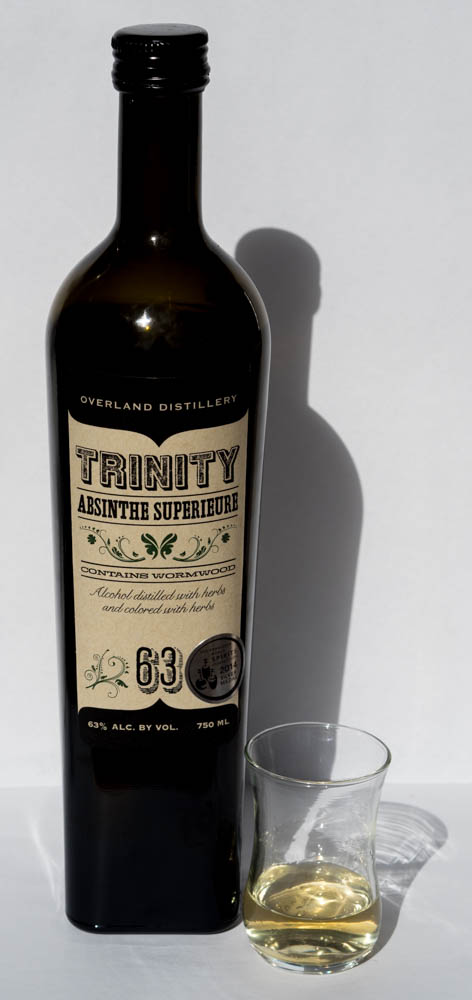
\includegraphics[width=\linewidth]{../../assets/tasting/naa-trinity.jpg}
  \end{wrapfigure}

  The color of the straight spirit is a greenish yellow, almost tan.  They defend the color of the product on their website as being totally natural (as any good absinthe should be).  It's not unpleasant, to be sure, but hardly the peridot one might be expecting when pouring from the dark bottle.

  When smelled straight, one is a little surprised by the relative lack of anise.  The nose is greeted with a vaguely savory smell as oregano and coriander dominate, along with plenty of angelica and wormwood.  There is a very faint odor of what I thought was heads at first -- heads are the first part of the distillation that contains a greater concentration of methanol and other solvents -- but over time that relaxes away.  I almost wonder if this was made with a grain alcohol rather than a grape alcohol.  As the empty nosing glass begins to evaporate, one can smell the anise more clearly.  It's still lighter than expected, but pleasant all the same.

  The downplayed anise and fennel is evident in the very mild louche, even at the relatively ``strong'' ratio of 3:1.  When water begins to drip into the absinthe, one can see the mixtures swirling rather like heat waves, as one might with any absinthe, but this never develops into the opalescence that I expect from more anise-heavy absinthes.  The faint louche picks up on the green notes from the straight spirit a little at least, and the color is appealing, if light, but the louche is too light for my tastes.

  When water is added and the absinthe smelled, I was struck almost immediately by the same savory notes from the straight spirit, joined by a smell of chlorine, as though I'd poolside.  This was so confusing that I dumped the first glass of absinthe out, rewashed my glass, and tried again.  The unpleasant odor was there again, making me mark that as a point against this absinthe.

  The flavor is as light as the color and the nose.  One is struck immediately with hot alcohol fighting against cooling anise.  The fennel becomes evident in the mid, with a bit of astringency from the more bitter herbs.  The anise and wormwood linger on the tail, along with an unpleasant whiff of chlorine from the back of the throat.  The body of the absinthe was similarly light, the mouthfeel coming across more like a vodka or gin than the fullness of many other absinthes.

  I tried once more with sugar, and was greeted by a more pleasant mouthfeel, much thicker, but more of the same in terms of flavors; I wasn't able to finish the sweetened glass.

  This was an intriguing absinthe.  It has flaws keeping it from being a wonderful drink on its own -- the note of chlorine being prime among them -- but I got the impression that this absinthe would work well when incorporated into a cocktail, such as the Absinthe cocktail or Sazerac listed below.

  \secdiv

  \section*{Absinthe and Pop Culture}

  \begin{wrapfigure}{r}{0.5\linewidth}
    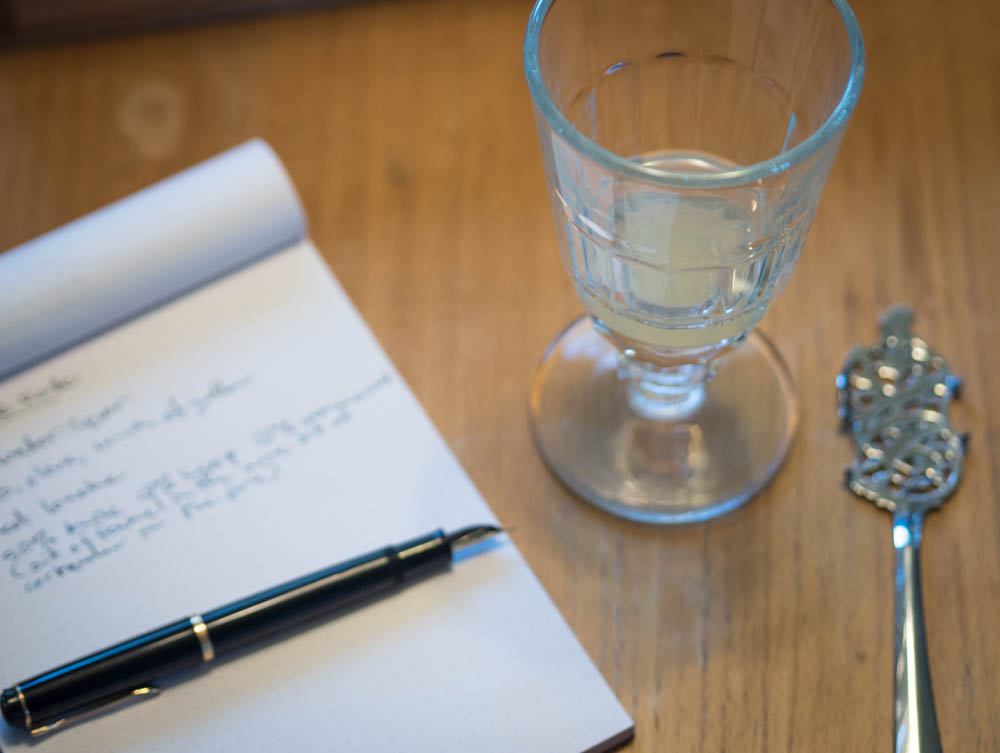
\includegraphics[width=\linewidth]{../../assets/tasting/naa-tasting.jpg}
  \end{wrapfigure}

  The combination of its popularity in the past, followed by its legal status in the 20th century left absinthe with something of an air of mystery.  Legends and myths surround the drink and wormwood specifically (many producers made pastis, an herbal drink featuring all of the ingredients of absinthe minus the wormwood, which only served to highlight the plant).  It was described as a hallucinogen, as poison, said that it would make you crazy and cut off your ear like van Gogh, that it would make you fall in love.

  Absinthe was, is, and will likely always be a relatively simple drug, however: alcohol.  That does nothing to stop the associations from forming in people's minds, nor indeed from corporations playing up those myths for the sake of sales.

  One of the pervasive perceptions around absinthe is that it is, to some extent, magical.  \textit{La F\'ee Verte}, people call it, the green fairy or the green muse.  It transports them on a magical ride from here to somewhere else; deep realms of the mind, perhaps, or strange planes of existence.  I certainly understand the roots of this: there is doubtless something unique and wonderful about absinthe, but something simple.  It's a drink that ``smell[s] like bottled summer'', it's calm, relaxing, something to sip slowly, something to ponder and enjoy.

  However, I think that one ought to be wary of fluff and marketing.  One must approach with a beginner's mind, at ground state. After all, this is what has led to that influx of awful Czech ``absinths'', and the hilarious (and dangerous) ``Czech ritual'' of pouring the ``absinth'' over the sugar cube and then lighting it on fire to let it drip down into the drink.  Needless to say, \textit{any} alcohol and fire is an awful idea, but one ought never do that with proper absinthe, unless one is keen only on destroying it.

  I repeat: No fire.

  Fire bad.

  You know, I think the impressionists, as mentioned above by Dale Pendell, had it right.  It wasn't some wacky trip to the moon, nor was it your mind being flooded by the unending truths of geometric shapes, nor even that it's simply alcohol.  It's light viewed through a delicate liquor that makes the world seem a little more full, a little more complete by its mere presence.

  Even I'm waxing poetic.

  \secdiv

  \section*{Vilya Spirits Absinthe Blanche}

  \begin{wrapfigure}{l}{0.38\linewidth}
    \vspace{-15pt}
    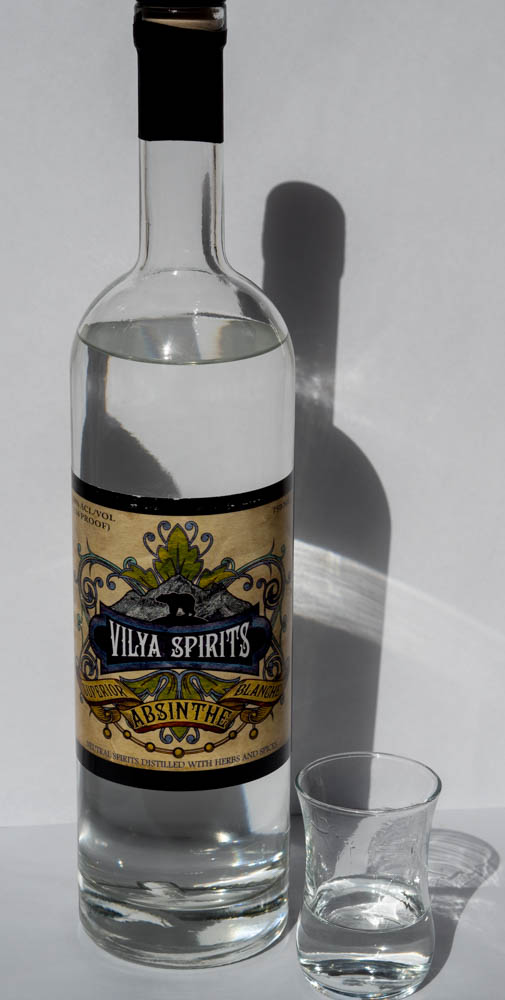
\includegraphics[width=\linewidth]{../../assets/tasting/naa-vilya-blanche.jpg}
    \vspace{-30pt}
  \end{wrapfigure}

  Not all absinthes are green, not by a long shot.  I'll go into some more details about that later, green absinthes are simply the most popular.  Needless to say, here is the only blanche absinthe on the list that I'm tasting.

  Vilya Spirits, which used to be named Ridge Distillery, is a distillery in Montana that focuses on herbal liquors and liqueurs, producing two absinthes, a gin, and a huckleberry liqueur, of which I've only tasted the absinthes.  I sought them about because they are some of the highest rated American absinthes on the Wormwood Society's reviews pages, and for good reason.

  The color of the undiluted spirit is bright and clear, a little finer than water or even vodka.  It smells delightfully of anise cookies, actually, as though someone were taking care in baking absinthe into a pastry.  There's a warmth, a sweetness that comes across with a little touch of vanilla.  As the nosing glass dries, the scent shifts over into a classic wormwood, fennel, and anise mix with a hint of coriander and angelica, really complex and delightful.

  The louche is quick and thick.  It starts out with a hint of blue as it begins to opalesce, then moves past opaline and into milky, cottony white, with just a hint of fading around the meniscus near the edges of the glass.  Watching the louche happen as the water drips into the glass is stunning.

  The baked goods come through a little in the diluted spirit as well, though in all, it's still definitely an absinthe.  There's plenty of anise and a bit of hyssop up front, fading to fennel and wormwood in the mid, then trailing off to cool anise and a touch of vanilla.  The mouthfeel is just about perfect on this, too, not too full, but certainly not flat.  It leaves the mouth just a touch dry, despite the sensation that the tongue and cheeks are coated in clean, licorice-y goodness, with a pleasant touch of numbing.

  When sugar is added, the cookie sense increases even further.  The added sugar batters down the hyssop, leaving primarily anise and fennel, with just a touch of vanilla.  I'm unsure of where that vanilla actually comes from, perhaps the angelica or maybe an addition of something else. Genepy, perhaps?  The resulting drink is almost perfect for dessert: it's not quite a candy, not quite a cookie, but the perfect end to a meal all the same.  Even fifteen minutes after drinking, I can still feel the slight coating of the mouth from the anise and the vague numbing effect, which is pleasant and comfortable.

  \secdiv

  \section*{Absinthe Preparation}

  \begin{wrapfigure}{l}{0.5\linewidth}
    \vspace{-15pt}
    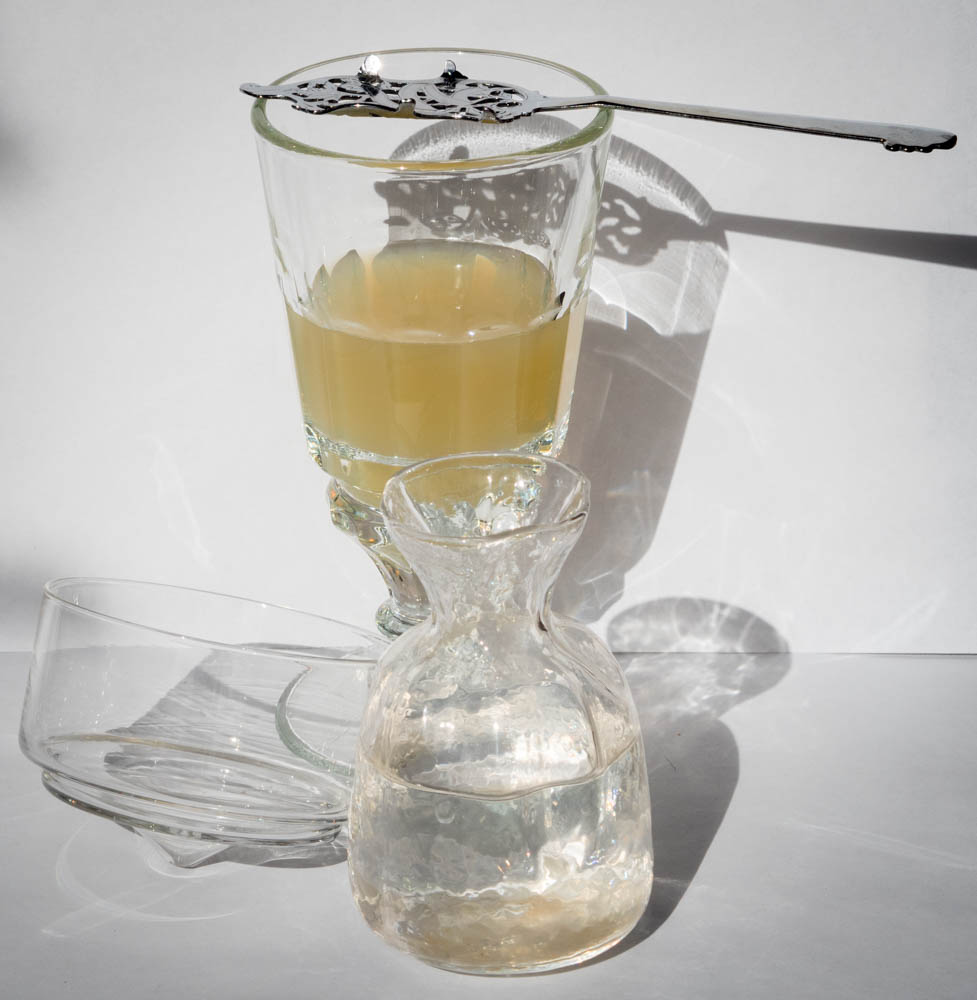
\includegraphics[width=\linewidth]{../../assets/tasting/naa-glassware.jpg}
    \textit{Proper glassware, including a dripper glass and Pontarlier glass, and a ``La Feuille'' style absinthe spoon.}
    \vspace{-50pt}
  \end{wrapfigure}

  The proper preparation of absinthe is very important and ought not to be ignored.

  One should use a proper Pontarlier glass.  This is a conical glass standing about as tall as a pint glass, with a rim similar in diameter.  However it's a stemmed piece of glassware, usually showing up as cut or molded glass.  There is a slight rim near the base of the bowl, showing the location to which one ought to fill with absinthe, leading to it's other name of a ``reservoir glass''.

  One should use at least cold, fresh tap water, if not spring water.  However, distilled water shouldn't be used.  It's important that the water be aerated, to have its oxygen content bulked up, otherwise the absinthe will taste flat and one dimensional.  The ratio of absinthe to water should start at 1:3, and then go up from there, to a max of 1:5 or 1:6, according to taste.

  The water should be iced prior to being added to the absinthe.  Although one may add ice to the final drink itself, it's not recommended, as the melting ice will change the dilution ratio and lead to a weaker drink at the end than at the beginning.

  Water should be added slowly to absinthe so as not to ``bruise'' the liquor.  This occurs when the droplets of terpenes held in suspension get knocked apart through overzealous addition of water, leading to a poor louche and poor flavor retention.

  Instead, you should introduce water to absinthe at a slow drizzle, either through the use of a dripper glass (my preferred method) or through an absinthe fountain.  Failing that, you can use a small measuring cup and pour the water gently and slowly down the side of the glass so as not to break up the absinthe too much.  The benefits of the fountain and the dripper glass is that you can fill them with ice before adding the water so that the water you use is as cold as it gets

  When it comes to sugar, I'm an advocate of at least trying the absinthe without sugar first, before trying it with sugar.  If you do decide that you prefer sugar, place a single sugar cube on the spoon and rest it atop the glass so that the water from the fountain drips over it.  If you are using a dripper glass, you can put the sugar cube in the conical section of the dripper glass before adding water.  I rather enjoy my absinthe with brown or Demerara sugar cubes, as they add a good deal of body and complexity, but even just white sugar will work.

  Despite all of this, absinthe is versatile, and can be used in many mixed drinks.  Here are a few of my favorites:

  \subsection*{The Absinthe Cocktail}

  \begin{itemize}[noitemsep]
    \item 1 part absinthe
    \item 1 part gin
    \item 1 part water
    \item 1 dash bitters
    \item Optional dash simple syrup
  \end{itemize}

  Shake or stir and serve in an absinthe glass.  The louche will be light, and tinged pink or orange from the cocktail bitters.  Garnish with a slice of orange.

  \newpage

  \subsection*{The Sazerac}

  \begin{itemize}[noitemsep]
    \item 1 sugar cube
    \item 2$\frac{1}{2}$ ounces rye whisky
    \item 2 dashes Peychaud's bitters
    \item 1 dash Angostura bitters
    \item absinthe
    \item lemon peel
  \end{itemize}

  In the bottom of an Old Fashioned glass, muddle the sugar cube with a few drops of water.  Add ice, the whiskey, and the bitters and stir.  Take a second Old Fashioned glass and swirl some absinthe around in it before pouring out (or back into the bottle, if you're positive your glass was clean).  Strain the cocktail into the absinthe-coated glass and serve with a twist of lemon.

  \subsection*{The Absinthe Suissesse}

  \begin{itemize}[noitemsep]
    \item 1$\frac{1}{2}$ oz absinthe
    \item $\frac{1}{2}$ oz orgeat syrup
    \item 1 egg white
    \item $\frac{1}{2}$ oz single cream
    \item shaved or crushed ice
  \end{itemize}

  Blend all ingredients in a blender for a few seconds and serve in a chilled cocktail glass.  Perfect for brunch.

  \secdiv

  \section*{St George Spirits Absinthe Verte}


  When I saw that \href{http://www.stgeorgespirits.com/}{St. George} was making an absinthe, I had to jump on it.

  I was lucky enough to visit this distillery, famous for being located in an old hangar in Alameda, CA (and thus for making Hangar One vodka there, though that's a different label) with my partner and a few friends.  The building is enormous, the tour guides well informed and funny, and all of their spirits delightful.  They're notable for their vodka, of course -- for them, I break my  ``no flavored vodkas'' rule; the blueberry and citron are heavenly -- but also for their gin with a focus on terroir and their eau de vie.

  \begin{wrapfigure}{r}{0.4\linewidth}
    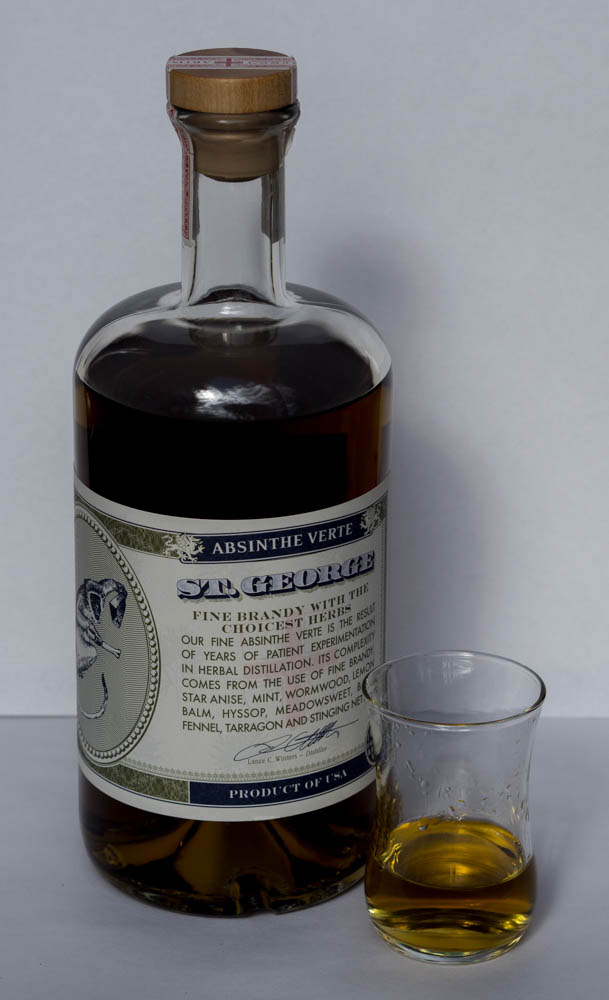
\includegraphics[width=\linewidth]{../../assets/tasting/naa-st-george.jpg}
  \end{wrapfigure}

  The absinthe itself is green, but hued towards olive, which may be in part due to the clear bottle: both Leopold Bros. and St. George absinthes tend closer to yellow, which can be due to being light-struck.  Hardly a huge flaw, though.

  The smell of the straight spirit is hot alcohol in the lead, followed by anise, fennel, and a surprising honey note, as if someone had blended in some tupelo honey.  There's not really any wormwood or any of the fuller herbs present in the nose, but once the glass dries a bit, you can pick up a bit of hyssop.

  The absinthe louches right in the middle of the road.  It's green and opaline without the olive tinge, neither thick nor thin, neither fast nor slow.  It reminds me rather a lot of the Jade absinthes, which leads me to want to call it ``typical'', though I may be off.

  The flavor of the diluted spirit explodes with sweetness, and really doesn't need sugar at all.  It leads with honey, then plenty of anise and star anise.  That flows into a bit of wormwood and fennel in the mid, followed by more cooling anise.  There's a gentle pinch of hyssop in the throat after, and the mouth is left with sweetness.  The smell is almost like someone blended honey with absinthe herbs.

  Adding sugar just seems to complete the transformation to honey.  Although the mouthfeel was fine for the drink without sugar, it gets even fuller with sugar, which may be adding to the sense of honey.  In fact, it reminds me of getting licorice-flavored honey sticks, right down to the slight tickle in the throat that eating plain honey can create.  That said, it's too sweet for me, with sugar.  It's wonderful without!

  \secdiv

  \newpage

  \section*{Absinthe Production}

  \begin{wrapfigure}{l}{0.5\linewidth}
    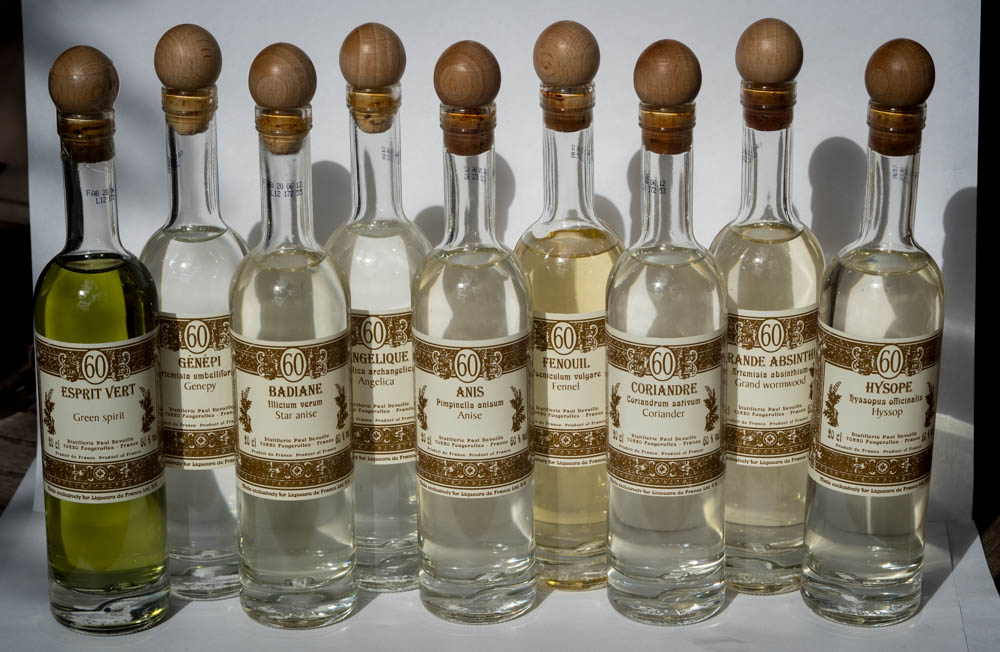
\includegraphics[width=\linewidth]{../../assets/tasting/naa-blends.jpg}
    \textit{Although most absinthes are produced through distillation and maceration as outlined below, the individual herbs can be macerated and distilled, and the resulting distillates blended into absinthes.  I've used them below to provide notes on the individual herbal ingredients.}
  \end{wrapfigure}

  Absinthe is a distilled spirit.  That is, after fermentation, the alcohol (or ``wash'') is heated very slowly in a mostly enclosed container called a still.  As the wash heats up, the alcohol evaporates first, leaving behind the water and other components that boil at a higher temperature.  The alcohol vapors travel up a column.  Once they get to the top, the building pressure pushes them down a pipe which is cooled somehow (``lyne arm'' and ``condenser''), usually with a cold water bath.  When the vapor cools down, it condenses on the inside of the pipe and drips out the end, much stronger than when it went in.

  This produces the base spirit.  With absinthes, this is often, though not always, grape spirit, which is the same sort of thing that might one day go to become brandy.  However, rather than aging it in oak for years, the grape spirit is collected, and a special selection of herbs are soaked (``macerated'') in it.  The alcohol leaches out all of the alcohol soluble compounds and flavors.  This mix is distilled once more.  If the absinthe is to be a \textit{verte} or green absinthe, there is one last step of maceration with select plants.  For \textit{blanche} or white absinthe, no last step is taken, and it's ready to bottle.

  This describes the primary means of producing absinthe, but another, simpler way to come up with different flavors and products is to go through the above process only for \textit{individual} herbs.  This way, you wind up with a distillate of just, say, anise or wormwood.  You can then blend these distillates together until you get a flavor that you like, then produce that at scale, either through blending or the maceration process.  If a second maceration step is not used but a green absinthe is desired, one may add \textit{esprit verte}, or green spirit, to color the absinthe.  This is an absinthe-like liqueur with mild flavor that will not affect the flavor of the blend much.

  What follows are some of the herbs and spices used in the creation of absinthe, their compounds of note, their effects on louche, and the smell and taste of the distillates of the single herbs.

  \subsection*{The ``Holy Trinity''}

  Absinthe simply isn't absinthe without these three.  They combine to form most of the aspects of the drink, from the smell and flavor to the louche and mouthfeel.

  \begin{description}[noitemsep]
      \item [Grand wormwood (\textit{Artemisia absinthum})] \hfill \
        \begin{description}[noitemsep]
          \item [Smell] herbal and fresh, reminiscent of bay or sage.
          \item [Taste] cooling and herbal, touch of bitterness, and some lingering sweetness, with just a touch of mint.
          \item [Effect on louche] none.
          \item [Compounds] $\alpha$-thujone, $\beta$-thujone, sabinene, myrcene, tras-sabinol, trans-sabinyl acetate, linalyl acetate, geranyl propionate.
      \end{description}
      \item [Fennel (\textit{Foeniculum vulgare})] \hfill \
        \begin{description}[noitemsep]
          \item [Smell] sweet aniseed with vegetal celeriac notes.
          \item [Taste] sweet and spicy with a bit of bitterness, some licorice flavors showing through toward the end through the vegetal aspects with mild numbing.
          \item [Effect on louche] medium.
          \item [Compounds] $\alpha$-pinene, myrcene, fenchone, trans-anethole, methyl chavicol, limonine, 1,8-cineole, anasic aldehyde.
      \end{description}
      \item [Anise (\textit{Pimpinella anisum})] \hfill \
        \begin{description}[noitemsep]
          \item [Smell] sweet and spicy, rather like licorice but less earthy and full, and more fresh.
          \item [Taste] very sweet, numbing, coating the mouth with a spicy, licorice-like sweetness without being cloying.
          \item [Effect on louche] strong.
          \item [Compounds] $\alpha$-pinene, $\beta$-pinene, camphene, linalool, cis-anethole, trans-anethole, safrole, anisaldehyde, acetoanisole
      \end{description}
  \end{description}

  \subsection*{Other ingredients}

  Absinthe can be made solely with the ``Holy Trinity'' ingredients, but it often lacks depth.  This can be achieved through the addition of various other herbs and ingredients to create a more unique experience.

  \begin{description}[noitemsep]
      \item [Genepy (\textit{Artemisia genipi}, \textit{Artemisia umbelliformis}, or \textit{Artemisia rupestris})] \hfill \
      \begin{description}[noitemsep]
          \item [Smell] vegetal and herbal, a touch of cinnamon and radish.
          \item [Taste] bitter and fresh like a radish, with only just a hint of sweetness, the cinnamon only showing through at the very end.
          \item [Effect on louche] none.
          \item [Compounds] $\alpha$-thujone, $\beta$-thujone, cineole, borneol, $\beta$-pinene
      \end{description}
      \item [Angelica (\textit{Angelica archangelica})] \hfill \
      \begin{description}[noitemsep]
          \item [Smell] bittersweet and vegetal, with notes of celeriac or celery leaves.
          \item [Taste] bittersweet and antiseptic, with a touch of astringency, the celery notes mostly in the fore.
          \item [Effect on louche] none.
          \item [Compounds] $\alpha$-pinene, $\beta$-pinene, camphene, sabinene, $\alpha$-phellandrene, $\beta$-phellandrene, myrcene, limonene, cis-ocimene, trans-ocimene, p-cymene, terpinolene, copaene, bornyl acetate, terpinen-4-ol.
      \end{description}
      \item [Star anise (\textit{Illicium verum})] \hfill \
      \begin{description}[noitemsep]
          \item [Smell] strong aniseed flavor similar to anise, but a little more vegetal and sweet.
          \item [Taste] intensely sweet and numbing, with a fresh aniseed flavor.  The vegetal note doesn't come through, but is almost overwhelmed by the spicy, cloying sweetness.
          \item [Effect on louche] very strong, often used to help with thicker louche.
          \item [Compounds] anethole, $\alpha$-pinene, philandrene, p-cynene, 1,4-cineol, limonene, d-turpenol.
      \end{description}
      \item [Hyssop (\textit{Hyssopus officianalis})] \hfill \
      \begin{description}[noitemsep]
          \item [Smell] astringent, bitter, and fresh, with notes of green tea.
          \item [Taste] astringent and bitter, a hint of spice coming through at points before fading into sweet and spicy vegetal and antiseptic notes.
          \item [Effect on louche] none.
          \item [Compounds] $\alpha$-pinene, $\beta$-pinene, camphene, sabinene, myrcene, limonene, pinocamphone, isopinocamphene, y-terpinol, 1,8-cineol, thujone.
      \end{description}
      \item [Coriander (\textit{Coriandrum sativum})] \hfill \
      \begin{description}[noitemsep]
          \item [Smell] spicy and savory, a lingering pleasant sweetness, reminiscent of carrots or jicama.
          \item [Taste] spicy and cooling, a touch astringent, very herbal and fresh.
          \item [Effect on louche] medium.
          \item [Compounds] Borneol, linalool, cineole, cymene, terpineol, dipentene, phellandrene, pinene, terpinolene.
      \end{description}
      \item [Other less-common additions] \
      Every absinthe recipe is different, and the herbs used are the primary ways of changing things up.  If one wants to aim for more sweetness, or more bitterness, or more freshness, one can add just about any herb or spice that one can think up.  These are just a few.  Of note, although absinthe is usually described as having a licorice flavor, actually using licorice isn't very common, with the flavor coming from anise or star anise.  Some examples would be: Calamus (\textit{Acorus calamus}), melissa (\textit{Melissa officianalis}), mint (\textit{Mentha spp.}), citron (\textit{Citrus medica}), or licorice (\textit{Glycyrrhiza glabra}).
  \end{description}

  Evaluating the ingredients based on their distillates is of the utmost importance, as ought to be shown by the Czech ``Absinth'' macerations.  Both wormwood and hyssop are shockingly bitter on their own.  In fact, wormwood contains absinthin, the second most bitter compound known.  Making a tea from wormwood, one would be hard pressed to enjoy it, or even stomach it.  However, when distilled, wormwood bursts forth with freshness, cooling sensations, and touches of mint.

  This is why really good absinthes go through all those steps of maceration and redistillation: the flavors that the producer is aiming for aren't contained in the maceration.  This is also why one must be very careful with the herbs used in the coloring step with verte absinthes, lest one introduce bitterness that one doesn't want.

  \secdiv

  \section*{Vilya Spirits Absinthe Verte}

  Alright, I'm going to come clean up front, here.  This is my favorite absinthe of the lot (though the St. George comes in a close second).

  We already tried the blanche absinthe, and talked about the difference between blanche and verte absinthes.  The difference between this absinthe and the blanche is clear from the start.  The color is a perfect peridot green, typifying the beautiful absinthes I tried from Jade.  It looks spectacular in the nosing glass.

  The smell is anise, fennel, and stone fruit to start.  Eventually, a bit of the base spirit -- grain spirits in this case -- shows through, with fantastic attention paid to the cuts.  This fades to a clean finish with what smells like a bit of coriander and melissa.

  The louche is another ``typical'' one, with medium speed and intensity: it's not as cottony as the blanche, but neither is it thin by any stretch.

  When water is added, the smell is relatively light, with bits of anise and angelica.  The taste is a perfect balance of bitter and sweet, without any astringency to speak of.  This leads with fresher herbs, rather like hyssop (though that isn't listed as an ingredient), coriander, and a judicious amount of anise.  It's not punchy at all.  The mid is warm wormwood and fennel, with some angelica peeking through, while the tail is a splash of bright, pleasant bitterness.  The coating that the sip leaves in your mouth is just as balanced as the drink: complex, rather than one-note anise.

  \begin{wrapfigure}{r}{0.4\linewidth}
    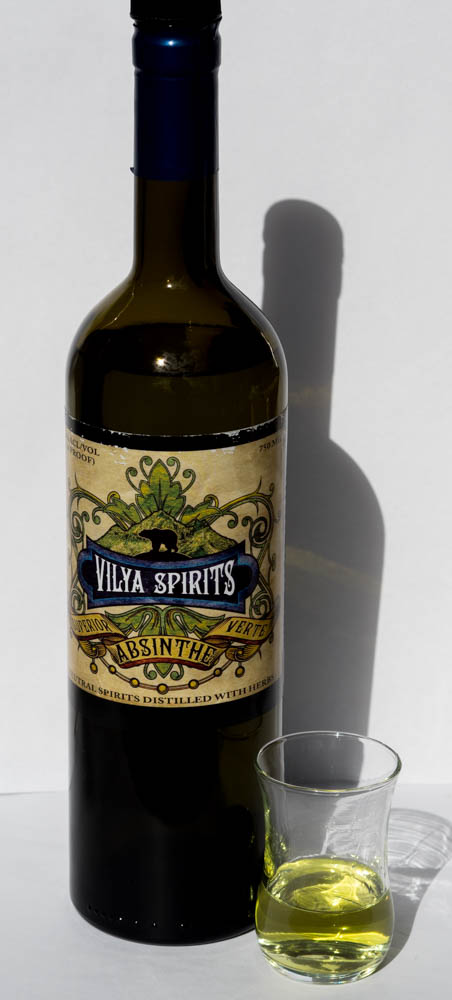
\includegraphics[width=\linewidth]{../../assets/tasting/naa-vilya-verte.jpg}
    \vspace{-50pt}
  \end{wrapfigure}

  When sugar is added, the wormwood and coriander are mulled almost totally, but not completely gone.  The absinthe remains wonderfully complex, though some of the admirable (to me) qualities are lost to the sugar.  Even so, this absinthe does well with the addition of sugar, not turning into simple anise candy.

  Of all of the absinthes that I tasted for this article, this was the clear winner, far and away.  Everything about it screamed ``absinthe''.  The color was spot on, the louche was simply the type for the class, and the flavor started by taking me back to those first sips of French absinthe, and then went so far above and beyond them, perfect with or without sugar.  It's my favorite, I'm not ashamed to say, and I can't recommend it highly enough.

  \secdiv

  \section*{Absinthe and Craft Spirits}

  In the years of World War I and prohibition, all but the strongest of breweries were shut down, with their tuns and kettles repurposed for the war effort.  Even the strongest breweries, no longer allowed to make beer, had to retool and repurpose their equipment or else be shuttered.

  In 1933, when prohibition was repealed, many celebrated the reopening of the breweries.  However, the law had taken its toll: the number of American breweries had declined nearly into the single digits.  There was Anheuser-Busch, Schlitz, Miller, and not a whole lot else.  None of the smaller breweries had been able to weather the dry (well, ``dry'') years.

  Without competition, the remaining breweries flourished and prospered.  There was no reason to compete on flavor or inventiveness.  The only real competition was over price.  To reduce costs, the big breweries began to find ways to make beer cheaper to manufacture.  The introduction of rice and corn were a big step in that direction.

  After the 21st amendment was passed, homebrewing was still illegal.  It wouldn't be until 1978 when a dedicated core group of folks brewing at home finally got homebrewing legalized on a federal level, though some states kept laws on their books about brewing one's own beer.

  \begin{wrapfigure}{l}{0.5\linewidth}
    \vspace{-15pt}
    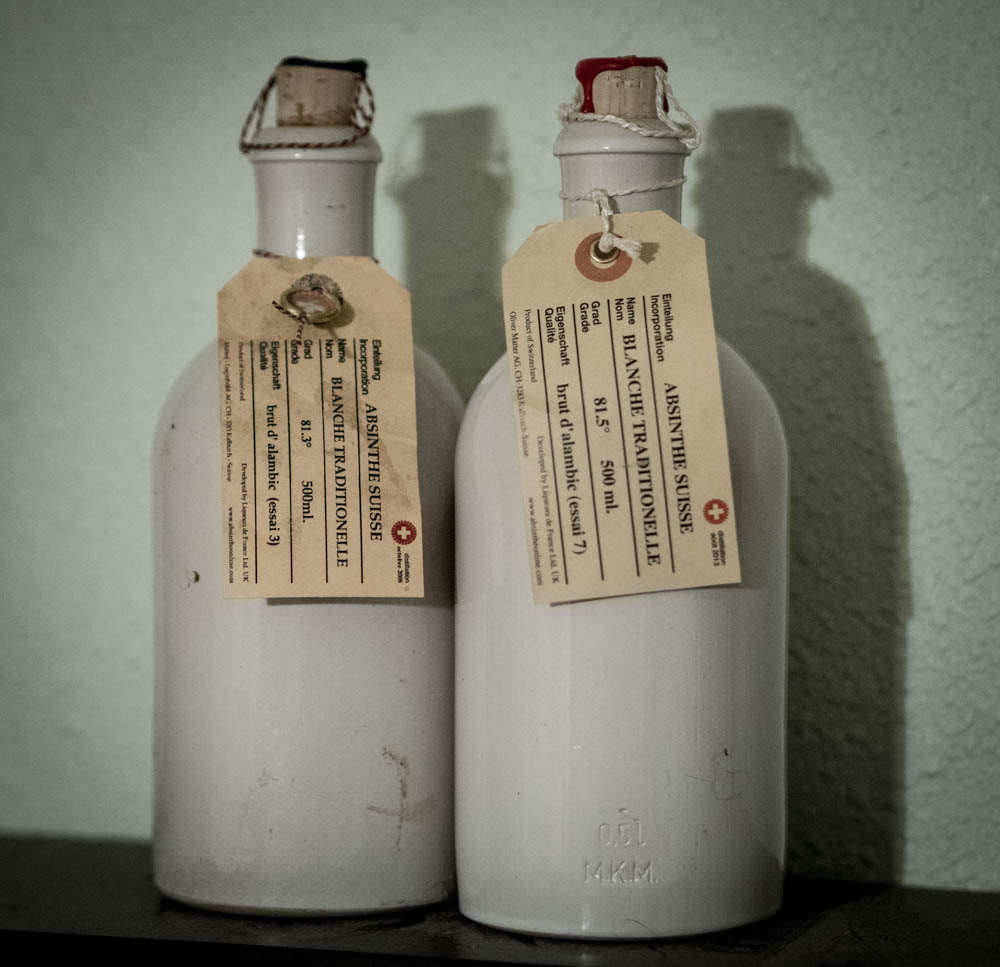
\includegraphics[width=\linewidth]{../../assets/tasting/naa-essai.jpg}
    \textit{Brut d'Alembic Assays (cask-strength tests) used for perfecting a recipe; the final recipe will go into mass production, but these assays are sold in limited quantities.}
    \vspace{-15pt}
  \end{wrapfigure}

  The widespread result of this legislation wouldn't be felt for some time.  It would take time for equipment and materials to become useable by the amateur.  It would take time for the amateur to learn the craft.  It would take time for the amateur to work to becoming a professional.

  After some years, though, one began to see more and more brew pubs, and more and more of a new kind of brewery: the microbrewery.

  The microbrewery was seen as the extension of homebrewing into a market.  Microbreweries, seen as premium, could charge a premium for their product, and thus had more freedom to experiment with styles.  Ales started becoming popular again.  We started seeing the creation of an American beer aesthetic: somewhere in the land of India pale ales, yet focusing on citrusy American hops and darker malts.

  By the turn of the century, one started to see these microbreweries growing to the size where they could hardly be called micro anymore.  They had interstate distribution, recognizable brand names, and many different branch breweries.  However, the premium remained, as did the experimentation to some extent.  One started to hear about ``flagship beers'', such as Sam Adams' Boston Lager, or New Belgium's Fat Tire.

  There needed to be a new term for these breweries that were larger than microbreweries but held to their micro roots.  The term that was settled on was craft breweries.

  Now, the craft distillery movement did not follow this trajectory.  Distilling at home is still decidedly illegal, unless one gets a fuel ethanol permit.  Setting up a distillery is much harder than a brewery, too.  One needs most of the equipment needed for a brewery -- a mash tun, a fermentation vessel, storage tanks, aging vessels and so on -- plus the still.  If one is aiming to produce cask-aged spirits, then one also needs casks and space to age.  Plus, if one is aiming to make anything other than neutral spirits such as vodka or white rum, one needs time.  Lots and lots of time.  The minimum age for a bourbon is two years; that's two years where you can't sell it and make back the money that you invested into it.

  What the craft distilling industry appears to have done is taken inspiration from the microbrewery industry and run with it.  Many followed the same pattern of creating a vodka or light rum at first, and then broadening their selection by creating liqueurs, sometimes rotating different flavors in and out, while their liquors aged in barrels.  Later on, they could add whiskeys and brandies to their lineups.

  Herbal liqueurs began to crop up here and there, and as soon as the regulations on absinthe were clarified in 2007, absinthes immediately began to show up as well.

  One thing that we're starting to see with breweries, now, is market saturation.  The selection at any given liquor store is overwhelming, to the point where many offer ``mix-and-match six-packs'', allowing customers to try six individual beers for a set price.  Another side effect of this is that we are starting to see regional, local, and hyperlocal breweries producing beers, leaning back on the brewpub model, or even getting close to the independent pub model that one sees in other countries: a place that serves beer that it makes, perhaps a cheese plate, and not a whole lot else (this is called a tavern license in Colorado, and may be similar elsewhere).

  Will we start to see the same thing, in general with craft spirits, or specifically with absinthe?  I don't know, I can't honestly say.  However, I do think that it's important to think critically about the things that we enjoy this way, because this feels like a very American problem to be facing.  That entrepreneurship would lead to a flooded market is certainly a global problem, but the way in which it has happened in craft alcohols, the very speed by which it has turned into an industry watched by venture capitalists feels uniquely us.  We take something exciting and jump on it and do all sorts of crazy things, sometimes bad, sometimes good.  Absinthe over here is one of those things.

  I don't think it's bad, per se, though getting started into drinking \textit{any} particular tipple is tough, when the selection is so wide.  I think back to my introduction to scotches and wines.  About how I felt the need to really go all out and explore \textit{everything}.  I burned out pretty quickly, however, and burning out is an expensive proposition.

  In the end, however, I fell back on what my good friend and bartender, Raffi Jergerian, taught me.  Raffi studied forestry and ecology, traveled to Italy to study wine, and eventually came home to become a sommelier.  After a while, though, he left to become head bartender at a small, upscale bar, then moved on to help open a bar to call his own in Fort Collins.

  Why the move to spirits and mixed drinks?  ``Explore a little, sure,'' he said. ``Then find what you like to drink and drink that.''

  Wise words.  Drink well.

  \newpage

  \section*{Notes}

  If, after all of this, you're still keen on absinthe and want to learn more, there are quite a few resources available for you out there.  First and foremost, I'd recommend checking out the \href{wormwoodsociety.org}{Wormwood Society}, a group who is dedicated to promoting and expanding the world of absinthe.  Their reviews are notable for being extensive and well thought out.  They make a wonderful resource.

  Much of my technical information came from the book \textit{Pharmako/Poeia}, by Dale Pendell.  The \textit{Pharmako Trilogy} are three wonderful books about the way we perceive plants of power, as well as the way that they shape society.  From coffee and tea to alcohol and marijuana, the author weaves a poetic and informative journey through interesting and sometimes scary plants and substances.

  The herbal distillates that I used for describing the component herbs used in making absinthe came from \href{http://www.absintheonline.com/acatalog/Absinthe_Blending_kit.html}{Liqueurs de France}, which is also where I got my Jade absinthes.  Most of the distillates come as a set in a lovely wooden box, with three additional bottles being offered for assaying.  They are nominally used for blending one's own absinthe to taste, but I think they're wonderful for ascertaining what all goes into an absinthe.

\end{document}
